\documentclass[10pt,a4paper]{amsart}
\usepackage{amsmath,amssymb,amsthm,graphicx}
% Class-compatibility preamble for a reader excerpt of
%   Masuda-Thomas-Tonks-Vallette, "The diagonal of the associahedra", JEP 8 (2021), DOI 10.5802/jep.142.
%
% This file is the source directory's inherited layout adapter, unchanged except for one
% mechanical line: \smaller is declared with \providecommand instead of \newcommand because the
% wrapper class used for this excerpt (amsart) already defines \smaller as a font-size command.
% No mathematical macro, statement or proof step is added.
\usepackage{amsmath,amssymb,amsthm,xfrac,xspace,hyperref,graphicx,comment}
\excludecomment{DefTralics}

\providecommand{\bibliofont}{\small}
\newcommand{\ie}{i.e.,\xspace}
\newcommand{\eg}{e.g.,\xspace}
\newcommand{\etc}{etc.\xspace}
\newcommand{\cf}{cf.\xspace}
\newcommand{\resp}{resp.\xspace}
\providecommand{\smaller}{\small}
\newcommand{\Subsection}{\subsection}
\newcommand{\Subsubsection}{\subsubsection}
\newcommand{\skpt}{\smallskip}
\emergencystretch=3em
\numberwithin{equation}{section}\providecommand{\No}{}
\usepackage{mathrsfs}
\let\mathcal\mathscr
\usepackage{mathtools}
\newcommand{\Changel}{\mathcode`l="7160}
\newcommand{\Changelback}{\mathcode`l="716C}
\newcommand{\NoChangel}[1]{%
\expandafter\let\csname old\string#1\endcsname=#1
\let#1=\relax
\newcommand{#1}{\mathcode`l="716C\csname old\string#1\endcsname\mathcode`l="7160 }%
}
\def\mto{\mathchoice{\longmapsto}{\mapsto}{\mapsto}{\mapsto}}
\def\hto{\mathrel{\lhook\joinrel\to}}
\def\ltwoheadrightarrow{\longrightarrow\hspace*{-5mm}\longrightarrow}
\def\stwoheadrightarrow{\rightarrow\hspace*{-3mm}\rightarrow}
\def\twoheadrightarrow{\mathchoice{\ltwoheadrightarrow}{\stwoheadrightarrow}{\stwoheadrightarrow}{\stwoheadrightarrow}}
\def\To#1{\mathchoice{\xrightarrow{\textstyle\kern4pt#1\kern3pt}}{\stackrel{#1}{\longrightarrow}}{}{}}
\def\Hto#1{\mathrel{\lhook\joinrel\To{#1}}}
\newcommand{\sbullet}{{\scriptscriptstyle\bullet}}

\NoChangel{\log}
\NoChangel{\ln}
\NoChangel{\lim}
\NoChangel{\limsup}
\NoChangel{\liminf}
\NoChangel{\varlimsup}
\NoChangel{\varliminf}
\NoChangel{\varinjlim}
\NoChangel{\varprojlim}

\let\dpl\displaystyle
\let\ts\textstyle

\AtBeginDocument{%
\def\labelitemi{$\sbullet$}%
}

\usepackage{graphicx}
\usepackage{multirow}

\usepackage[noabbrev,capitalize]{cleveref}
\crefdefaultlabelformat{#2\textup{#1}#3}

\usepackage{tikz}
\usepackage{tikz-cd}
\tikzset{math3d/.style=
{x= {(-0.353cm,-0.353cm)}, z={(0cm,1cm)},y={(1cm,0cm)}}}
\tikzset{JLL3d/.style=
{x= {(0.4cm,-0.2cm)}, z={(0cm,1cm)},y={(-1cm,0cm)}}}

\theoremstyle{plain}
\newtheorem{proposition}{Proposition}
\newtheorem{theorem}{Theorem}
\newtheorem*{problem}{Problem}
\newtheorem{corollary}{Corollary}
\newtheorem{lemma}{Lemma}
\newtheorem{conjecture}{Conjecture}

\theoremstyle{definition}
\newtheorem{definition}{Definition}
\newtheorem{remark}{Remark}
\newtheorem{example}{Example}

\newcommand{\RR}{\mathbb{R}}
\newcommand{\ZZ}{\mathbb{Z}}
\newcommand{\ZP}{\mathbb{Z}_{>0}}
\newcommand{\K}{{K}}
\newcommand{\La}{\mathcal{L}}
\newcommand{\Tam}[1]{\mathrm{PBT}_{#1}}
\newcommand{\PT}[1]{\mathrm{PT}_{#1}}
\newcommand{\sC}{\mathcal{C}}
\newcommand{\PolySub}{\mathsf{Poly}}\NoChangel{\PolySub}
\newcommand{\Top}{\mathsf{Top}}
\newcommand{\CW}{\mathsf{CW}}
\newcommand{\sF}{\mathcal{F}}
\DeclareMathOperator{\tp}{top}
\DeclareMathOperator{\bm}{bot}
\DeclareMathOperator{\pr}{pr}
\DeclareMathOperator{\conv}{conv}
\DeclareMathOperator{\diam}{diam}
\newcommand{\ang}[1]{\langle #1\rangle}
\renewcommand{\No}{\mathcal{N}}
\newcommand{\Ve}{\mathcal{V}}
\newcommand{\Bool}[1]{\{0, 1\}^{#1}}
\newcommand{\sk}{\mathrm{sk}}
\DeclareMathOperator{\vol}{vol}\NoChangel{\vol}
\newcommand{\tr}{\mathrm{tr}}
\newcommand{\id}{\mathrm{id}}
\newcommand{\itd}[1]{\triangle^{(#1)}}
\DeclareMathOperator*{\colim}{\mathrm{colim}}
\DeclareMathOperator{\im}{\mathrm{Im}}
\newcommand{\abs}[1]{\lvert #1\rvert}
\DeclareMathOperator{\codim}{codim}

\newcommand{\TreeR}
{\vcenter{\hbox{
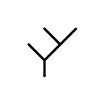
\begin{tikzpicture}[yscale=0.2,xscale=0.2]
\draw[thick] (0,-1)--(0,0) -- (2,2);
\draw[thick] (1,1)--(0,2) ;
\draw[thick] (0,0)--(-1,1) ;
\draw [fill] (0,-1) circle [radius=0.035];
\draw [fill] (2,2) circle [radius=0.035];
\draw [fill] (0,2) circle [radius=0.035];
\draw [fill] (-1,1) circle [radius=0.035];
\end{tikzpicture}}}}
\newcommand{\TreeL}
{\vcenter{\hbox{
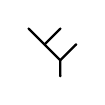
\begin{tikzpicture}[yscale=0.2,xscale=0.2]
\draw[thick] (0,-1)--(0,0) -- (-2,2);
\draw[thick] (-1,1)--(0,2) ;
\draw[thick] (0,0)--(1,1) ;
\draw [fill] (0,-1) circle [radius=0.035];
\draw [fill] (-2,2) circle [radius=0.035];
\draw [fill] (0,2) circle [radius=0.035];
\draw [fill] (1,1) circle [radius=0.035];
\end{tikzpicture}}}}
\newcommand{\TreeLL}
{\vcenter{\hbox{
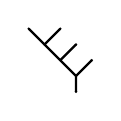
\begin{tikzpicture}[yscale=0.2,xscale=0.2]
\draw[thick] (0,-1)--(0,0) -- (-3,3);
\draw[thick] (-1,1)--(0,2) ;
\draw[thick] (-2,2)--(-1,3) ;
\draw[thick] (0,0)--(1,1) ;
\draw [fill] (0,-1) circle [radius=0.035];
\draw [fill] (-2,2) circle [radius=0.035];
\draw [fill] (0,2) circle [radius=0.035];
\draw [fill] (1,1) circle [radius=0.035];
\draw [fill] (-3,3) circle [radius=0.035];
\draw [fill] (-1,3) circle [radius=0.035];
\end{tikzpicture}}}}
\newcommand{\TreeLR}
{\vcenter{\hbox{
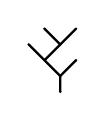
\begin{tikzpicture}[yscale=0.2,xscale=0.2]
\draw[thick] (0,-1)--(0,0) -- (-2,2);
\draw[thick] (-1,1)--(1,3) ;
\draw[thick] (0,0)--(1,1) ;
\draw[thick] (0,2)--(-1,3) ;
\draw [fill] (0,-1) circle [radius=0.035];
\draw [fill] (-2,2) circle [radius=0.035];
\draw [fill] (0,2) circle [radius=0.035];
\draw [fill] (1,1) circle [radius=0.035];
\draw [fill] (-1,3) circle [radius=0.035];
\draw [fill] (1,3) circle [radius=0.035];
\end{tikzpicture}}}}
\newcommand{\TreeRR}
{\vcenter{\hbox{
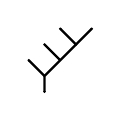
\begin{tikzpicture}[yscale=0.2,xscale=0.2]
\draw[thick] (0,-1)--(0,0) -- (3,3);
\draw[thick] (1,1)--(0,2) ;
\draw[thick] (2,2)--(1,3) ;
\draw[thick] (0,0)--(-1,1) ;
\draw [fill] (0,-1) circle [radius=0.035];
\draw [fill] (2,2) circle [radius=0.035];
\draw [fill] (0,2) circle [radius=0.035];
\draw [fill] (-1,1) circle [radius=0.035];
\draw [fill] (3,3) circle [radius=0.035];
\draw [fill] (1,3) circle [radius=0.035];
\end{tikzpicture}}}}
\newcommand{\TreeRL}
{\vcenter{\hbox{
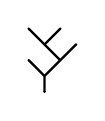
\begin{tikzpicture}[yscale=0.2,xscale=0.2]
\draw[thick] (0,-1)--(0,0) -- (2,2);
\draw[thick] (1,1)--(-1,3) ;
\draw[thick] (0,0)--(-1,1) ;
\draw[thick] (0,2)--(1,3) ;
\draw [fill] (0,-1) circle [radius=0.035];
\draw [fill] (2,2) circle [radius=0.035];
\draw [fill] (0,2) circle [radius=0.035];
\draw [fill] (-1,1) circle [radius=0.035];
\draw [fill] (1,3) circle [radius=0.035];
\draw [fill] (-1,3) circle [radius=0.035];
\end{tikzpicture}}}}
\newcommand{\TreeCC}
{\vcenter{\hbox{
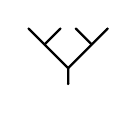
\begin{tikzpicture}[yscale=0.2,xscale=0.2]
\draw[thick] (0,-1)--(0,0) -- (-2.5,2.5);
\draw[thick] (-1.5,1.5)--(-0.5,2.5) ;
\draw[thick] (1.5,1.5)--(0.5,2.5) ;
\draw[thick] (0,0)--(2.5,2.5) ;
\draw [fill] (0,-1) circle [radius=0.035];
\draw [fill] (-2.5,2.5) circle [radius=0.035];
\draw [fill] (-0.5,2.5) circle [radius=0.035];
\draw [fill] (0.5,2.5) circle [radius=0.035];
\draw [fill] (2.5,2.5) circle [radius=0.035];
\end{tikzpicture}}}}
\newcommand{\TreeAL}
{\vcenter{\hbox{
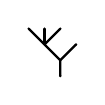
\begin{tikzpicture}[yscale=0.2,xscale=0.2]
\draw[thick] (0,-1)--(0,0) -- (-2,2);
\draw[thick] (-1,1)--(0,2) ;
\draw[thick] (0,0)--(1,1) ;
\draw[thick] (-1,1)--(-1,2) ;
\draw [fill] (0,-1) circle [radius=0.035];
\draw [fill] (-2,2) circle [radius=0.035];
\draw [fill] (0,2) circle [radius=0.035];
\draw [fill] (1,1) circle [radius=0.035];
\draw [fill] (-1,2) circle [radius=0.035];
\end{tikzpicture}}}}
\newcommand{\TreeRA}
{\vcenter{\hbox{
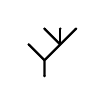
\begin{tikzpicture}[yscale=0.2,xscale=0.2]
\draw[thick] (0,-1)--(0,0) -- (2,2);
\draw[thick] (1,1)--(0,2) ;
\draw[thick] (0,0)--(-1,1) ;
\draw[thick] (1,1)--(1,2) ;
\draw [fill] (0,-1) circle [radius=0.035];
\draw [fill] (2,2) circle [radius=0.035];
\draw [fill] (0,2) circle [radius=0.035];
\draw [fill] (-1,1) circle [radius=0.035];
\draw [fill] (1,2) circle [radius=0.035];
\end{tikzpicture}}}}
\newcommand{\TreeAR}
{\vcenter{\hbox{
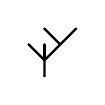
\begin{tikzpicture}[yscale=0.2,xscale=0.2]
\draw[thick] (0,-1)--(0,0) -- (2,2);
\draw[thick] (1,1)--(0,2) ;
\draw[thick] (0,0)--(-1,1) ;
\draw[thick] (0,0)--(0,1) ;
\draw [fill] (0,-1) circle [radius=0.035];
\draw [fill] (2,2) circle [radius=0.035];
\draw [fill] (0,2) circle [radius=0.035];
\draw [fill] (-1,1) circle [radius=0.035];
\draw [fill] (0,1) circle [radius=0.035];
\end{tikzpicture}}}}
\newcommand{\TreeLA}
{\vcenter{\hbox{
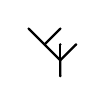
\begin{tikzpicture}[yscale=0.2,xscale=0.2]
\draw[thick] (0,-1)--(0,0) -- (-2,2);
\draw[thick] (-1,1)--(0,2) ;
\draw[thick] (0,0)--(1,1) ;
\draw[thick] (0,0)--(0,1) ;
\draw [fill] (0,-1) circle [radius=0.035];
\draw [fill] (-2,2) circle [radius=0.035];
\draw [fill] (0,2) circle [radius=0.035];
\draw [fill] (1,1) circle [radius=0.035];
\draw [fill] (0,1) circle [radius=0.035];
\end{tikzpicture}}}}
\newcommand{\TreeCA}
{\vcenter{\hbox{
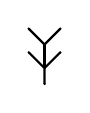
\begin{tikzpicture}[yscale=0.2,xscale=0.2]
\draw[thick] (0,-1)--(0,0) -- (-1,1);
\draw[thick] (0,1.5)--(1,2.5) ;
\draw[thick] (0,1.5)--(-1,2.5) ;
\draw[thick] (0,0)--(1,1) ;
\draw[thick] (0,0)--(0,1.5) ;
\draw [fill] (0,-1) circle [radius=0.035];
\draw [fill] (-1,1) circle [radius=0.035];
\draw [fill] (1,2.5) circle [radius=0.035];
\draw [fill] (-1,2.5) circle [radius=0.035];
\draw [fill] (1,1) circle [radius=0.035];
\draw [fill] (0,1) circle [radius=0.035];
\end{tikzpicture}}}}
\newcommand{\TreeC}
{\vcenter{\hbox{
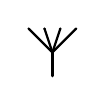
\begin{tikzpicture}[yscale=0.2,xscale=0.2]
\draw[thick] (0,-1.5)--(0,0);
\draw[thick] (0,0)--(1.5,1.5) ;
\draw[thick] (0,0)--(0.5,1.5) ;
\draw[thick] (0,0)--(-0.5,1.5) ;
\draw[thick] (0,0)--(-1.5,1.5) ;
\draw [fill] (0,-1.5) circle [radius=0.035];
\draw [fill] (1.5,1.5) circle [radius=0.035];
\draw [fill] (0.5,1.5) circle [radius=0.035];
\draw [fill] (-1.5,1.5) circle [radius=0.035];
\draw [fill] (-0.5,1.5) circle [radius=0.035];
\end{tikzpicture}}}}
\title{Existence, uniqueness and invertibility of the transition map between positively oriented polytopes with equivalent diagonal subdivisions}
\author{Naruki Masuda, Hugh Thomas, Andy Tonks, Bruno Vallette}
\date{doi:10.5802/jep.142; CC BY 4.0}
\begin{document}
\maketitle
\setcounter{proposition}{6}
\noindent\textit{Editorial note.} All delivered mathematical text and the native TikZ figures are the authors' own, copied from the fixed publisher source; the proof appears exactly as printed, including the enclosing enumerate, and nothing was rewritten or removed.\par\medskip
\noindent\textit{Editorial note.} The publisher class cedram is replaced by a plain wrapper for this excerpt: the preamble is the source directory's existing class-compatibility adapter together with the authors' own macros, with the single mechanical change that the short macro smaller is declared with providecommand, since the wrapper class already defines it as a font-size command. No mathematical macro was introduced.\par\medskip
\noindent\textit{Editorial note.} The environment number printed here continues the authors' own per-type counter, so the statement appears as the seventh proposition of the article; its source label is prop:Transition (source line 1166).\par\medskip
\noindent\textit{Editorial note.} Context blocks are the source definitions and the two earlier source results quoted by the proof (combinatorial equivalence and the category PolySub, positively oriented polytopes, the diagonal, Lemma:DiagOnFace, the coherent-subdivision construction, coherent/tight subdivisions, cor:DIMENSION); they are marked as context, not as this task's counted proof.\par\medskip
\noindent\textit{Allowed standard prerequisites (editorial).}\begin{itemize}
\item Elementary convex polytope topology: faces, skeleta, diameters and continuous maps on polytopes. Only standard facts are assumed: a continuous map on a polytope is determined by its values on a dense subset, and diameter estimates behave as usual. The iterated diagonal, the filtration P(n) and the continuity proof are retained obligations.
\item The category PolySub of polytopes with polytopal subdivisions and its isomorphisms. The definition of a morphism (a continuous map that is a homeomorphism onto the underlying set of a polytopal subcomplex with polytopal preimage) and of combinatorial equivalence is taken from the source excerpt; the claim that the constructed map is an isomorphism is proved, not assumed.
\item Notation for the diagonal of a positively oriented polytope and its restriction to faces. The excerpt carries the author's definition of triangle\_(P,v) and the author's proof that the diagonal of a face is the restriction of the diagonal of the polytope. Both are used verbatim by the retained proof at line 1211.
\end{itemize}\medskip
The face poset $\La(\sC)$ of a polytopal complex is defined in the obvious way.
We say that two polytopal complexes are \emph{combinatorially equivalent} when their face posets are isomorphic.
Now let us introduce the category we will work in.

\begin{definition}[The category $\PolySub$]
The category $\PolySub$ is made up of the following data.
\begin{itemize}
\item\emph{Objects}: An object is a $d$-dimensional polytope $P$ in the $n$-dimensional Euclidian space $\RR^n$, for any $0\leq d\leq n$.
\item\emph{Morphisms}: A continuous map $f: P\to Q$ is a morphism when
it sends $P$ homeomorphically to the underlying set $|\mathcal{D}|$ of a polytopal subcomplex $\mathcal{D}\subset \La(Q)$ of~$Q$
such that $f^{-1}(\mathcal D)$ defines a polytopal subdivision of $P$.
\end{itemize}
\end{definition}

There exists obvious forgetful functors from the category $\PolySub$ to the category $\Top$ of topological spaces with continuous maps and to the category $\CW$ of CW complexes with cellular maps. The latter functor is well-defined since any morphism in $\PolySub$ is automatically cellular.
An isomorphism $P\cong Q$ in this category is a cell-respecting homeomorphism which induces
a combinatorial equivalence $\La (P)\cong \La(Q)$.

\begin{definition}[Positively oriented polytope]
\begin{enumerate}
\item An \emph{oriented polytope} is a polytope $P\subset \RR^n$ endowed with a vector $\vec v\in \RR^n$ such that no edge of $P$ is perpendicular to $\vec v$, see \cref{Fig:PosOr}.
\begin{figure}[htb]
\[\vcenter{\hbox{
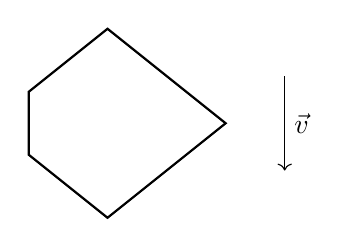
\begin{tikzpicture}[xscale=0.5, yscale=0.4]
\draw[thick] (0,3)--(-2,1)--(-2,-1)--(0,-3)--(3,0)--cycle;
\draw[->] (4.5,1.5)--(4.5,-1.5);
\draw (4.5,0) node[right] {$\vec v$};
\end{tikzpicture}
}}\]
\caption{An oriented polytope.}\label{Fig:PosOr}
\end{figure}

\item A \emph{positively oriented polytope} is an oriented polytope $(P, \vec v)$ such that the intersection polytope
\[
\big(P\cap \rho_z P, \vec v\big)
\]
is oriented, where $\rho_z\coloneqq 2z-P$ stands for the reflection with respect to any point $z\in P$, see \cref{Fig:Diag}.
\end{enumerate}
\end{definition}

The data of an orientation vector induces a poset structure on the set of vertices $\Ve(P)$ of $P$, which is the transitive closure of the relation induced by the oriented edges of the 1-skeleton.

\begin{definition}[Well-oriented realization of the associahedron]
A \emph{well-oriented reali\-zation of the associahedron} is a positively oriented polytope which realizes the associahedron and such that the orientation vector induces the Tamari lattice on the set of vertices.
\end{definition}

Before getting into specific argument on the associahedra, we construct a diagonal map $\triangle: P\to P\times P$ for any positively oriented polytope $(P, \vec v)$. Let $\tp_{\vec v} P$ (\resp $\bm_{\vec v} P$) denote the top (\resp bottom) vertex of $P$ with respect to the orientation vector $\vec v$.

\begin{definition}[Diagonal of a positively oriented polytope]\label{def:Diag}
The \emph{diagonal} of a positively oriented polytope $(P, \vec v)$ is defined by
\begin{align*}
\begin{array}{rlcl}
\triangle_{(P,\vec v)}\ : & P &\dpl\to &P\times P\\
&z & \dpl\mto&
\bigl(\bm_{\vec v}(P\cap \rho_z P),\, \tp_{\vec v}(P\cap \rho_z P)\bigr).
\end{array}
\end{align*}
\begin{figure}[htb]
\[
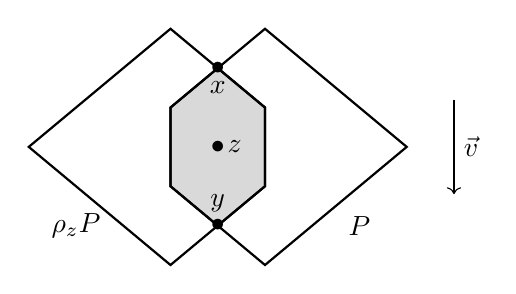
\begin{tikzpicture}[xscale=0.6, yscale=0.5]
\draw[thick] (1,3)--(-1,1)--(-1,-1)--(1,-3)--(4,0)--cycle;
\draw[thick] (-1,3)--(1,1)--(1,-1)--(-1,-3)--(-4,0)--cycle;

\draw[thick] (0,-2)--(-1,-1)--(-1, 1)--(0, 2)--(1, 1)--(1,-1)--cycle;
\draw[fill, opacity=0.15] (0,-2)--(-1,-1)--(-1, 1)--(0, 2)--(1, 1)--(1,-1)--cycle;

\draw[->] (5,1.2)--(5,-1.2);
\draw (5,0) node[right] {$\vec v$};
\draw (0,0) node {$\bullet$};
\draw (0,2) node {$\bullet$};
\draw (0,-2) node {$\bullet$};

\draw (0,0) node[right] {$z$};
\draw (0,1.9) node[below] {$x$};
\draw (0,-1.9) node[above] {$y$};

\draw (3,-2) node {$P$};
\draw (-3,-2) node {$\rho_z P$};
\end{tikzpicture}
\]
\caption{The diagonal map
$$\hspace*{-3cm}\triangle_{(P,\vec v)}(z)=\bigl(\bm_{\vec v}(P\cap \rho_z P),\, \tp_{\vec v}(P\cap \rho_z P)\bigr)=(x,y).$$}\label{Fig:Diag}
\end{figure}
\vspace*{-\baselineskip}
\end{definition}

Let $\beta$ be the middle-point map $P\times P\to P; (x,y)\mto \frac{x+y}{2}$.
With the notation $\pr_i$ for the projection to the $i$-th coordinate, we have $\pr_1\beta^{-1}(z)=\pr_2\beta^{-1}(z) = P\cap \rho_z P$.
The diagonal $\triangle_{(P,\vec v)}$ is a section of $\beta$ since $P\cap \rho_z P$ is symmetric with respect to the point $z$.

\begin{lemma}\label{Lemma:DiagOnFace}
Any face $F$ of a positively oriented polytope $(P,\vec v)$ is positively oriented once equipped with the orientation vector $\vec v$. Moreover, the two diagonals agree: $\triangle_{(P, \vec v)}(z)=\triangle_{(F, \vec v)}(z)$, for any $z\in F$.
\end{lemma}

\begin{proof}
This follows from the relation
$P\cap \rho_z P= F\cap \rho_z F$, for any $z\in F$.
\end{proof}

Let $\pi: Q\twoheadrightarrow P$ be an affine projection of polytopes with
$P\subset \RR^p$ and $Q\subset \RR^q$.
We~denote by $Q_z\coloneqq Q\cap \pi^{-1}(z)$ the fiber above $z\in P$.
To any linear form $\psi\in (\RR^q)^{\ast}$, we~associate a
collection
$\sF^\psi\subset \La(Q)$ as follows.
We first factor the affine projection~as\vspace*{-3pt}
\begin{align*}
\pi&=\mathrm{pr}\circ \tilde{\pi},& \text{where} \quad
\tilde{\pi}&\coloneqq (\pi, \psi): Q\twoheadrightarrow \tilde{P}\\
\tag*{and}
\mathrm{pr}&: \tilde{P}\twoheadrightarrow P;\, (z, t)\mto z,&
\text{where}\quad \tilde{P}&\coloneqq \big\{(\pi(x), \psi(x))\mid x\in Q\big\}\subset \RR^{p+1}.
\end{align*}
Next let $\La^{\downarrow}(\tilde P) \subset \La\big(\tilde{P}\big)$ be the subcomplex of lower faces, \ie $F\in \La^{\downarrow}(\tilde P)$ if and only if any $(z, t)\in F$ satisfies the equation
$t = \min \psi(Q_z)$. Since the preimage of any face by a projection of polytopes is again a face, this defines a collection\vspace*{-3pt}\enlargethispage{.5\baselineskip}%
\[\sF^\psi \coloneqq
\big\{Q\cap \tilde{\pi}^{-1}(F) \mid F\in \La^{\downarrow}(\tilde P)
\big\}
\subset \La(Q).\]
(This is in general not a polytopal complex since it is not stable under faces.)
In the case of the point $P=\{\ast\}$, the unique face contained in $\sF^\psi$ is by definition\vspace*{-3pt}
\[Q^\psi\coloneqq\{x\in Q \mid \psi (x) = \min \psi(Q)\}.\]

\begin{definition}[Coherent and tight subdivisions]\label{def:Coherent}
\begin{enumerate}
\item A subcollection $\sF\subset\La(Q)$ is called a \emph{coherent subdivision of $P$} when it is of the form $\sF^\psi$ for some $\psi\in (\RR^q)^{\ast}$.
\item A coherent subdivision $\sF$ is called \emph{tight} when, the faces $F$ and $\pi(F)$ have the same dimension, for every $F\in \sF$.
\end{enumerate}
\end{definition}

\begin{corollary}\label{cor:DIMENSION}
The image of $\triangle_{(P,\vec v)}$ is contained in $\sk_n (P\times P)$, where $n$ is the dimension of $P$. In particular, if one of two components of $\triangle (z)$ lies in the interior of $P$, then the other component is either $\tp_{\vec v} P$ or $\bm_{\vec v} P$.
\end{corollary}

\begin{proposition}\label{prop:Transition}
Let $(P, \vec v)$ and $(Q,\vec w)$ be two positively oriented polytopes, with a combinatorial equivalence $\Phi: \La(P)\xrightarrow{\cong} \La(Q)$.
Suppose that
tight coherent subdivisions
$\sF_{(P, \vec v)}$ and $\sF_{(Q, \vec w)}$ are combinatorially equivalent under
$\Phi\times \Phi$.
\begin{enumerate}
\item\label{prop:Transition1}
There exists a unique continuous map
\[\tr=\tr_P^Q : P\to Q,\]
which extends the restriction $\Ve(P)\to \Ve(Q)$ of $\Phi$ to the set of vertices
and which commutes with the respective diagonal maps.
\item\label{prop:Transition2} The map $\tr$ is an isomorphism in the category $\PolySub$, whose correspondence of faces agrees with $\Phi$.
\end{enumerate}
\end{proposition}

\begin{proof}
\begin{enumerate}
\item
In the core of this proof, we use the simple notation $\triangle_P$ for $\triangle_{(P, \vec v)}$ and
\[\triangle^{(n)}_P\coloneqq \triangle^{2^{n-1}}_P\circ \triangle^{2^{n-2}}_P\circ\cdots\circ\triangle^{2}_P\circ\triangle_P\ : \
P\to P^{2^{n}},\]
for its iterations.
We also denote the averaging map by
\begin{align*}
\begin{array}{rccc}
\beta^{(n)}_P\ : & P^{2^n}&\dpl\to &P\\
&(x_1, \ldots, x_{2^n}) & \dpl\mto&
\displaystyle \frac{x_1+\cdots+x_{2^n}}{2^n}.
\end{array}
\end{align*}
Notice that $\triangle^{(n)}_P$ is a section of $\beta^{(n)}_P$.
Any map $\tr$ commuting with the respective diagonal maps satisfies
\[\tr = \beta^{(n)}_Q\circ\tr^{2^n}\circ\triangle^{(n)}_P. \]

Let us prove the statement by induction on the dimension $d$ of the polytopes $P$ and $Q$. It is obvious for $d=0$. For $d=1$, let us suppose that $P=Q=[0,1]$ and that $\Phi(0)=0$, $\Phi(1)=1$, without any loss of generality.
Since the two polytopal subdivisions correspond bijectively under $\Phi$, the definition of the diagonal maps shows that $\vec v$ and $\vec w$ are oriented in the same direction. By dichotomy, one can check that the $2^n$-tuple $\triangle^{(n)}_P\left(\sfrac{k}{2^n}\right)$ is made up of $2^{n}-k$ zeros and $k$ ones. This induces the formula
\[\tr\left(\sfrac{k}{2^n}\right)
= \beta^{(n)}_Q\circ\Phi^{2^n}\circ\triangle^{(n)}_P\left(\sfrac{k}{2^n}\right)
= \sfrac{k}{2^n}. \]
The identity of $[0, 1]$ therefore provides the map $\tr$, and is unique by continuity.

Let us now suppose that the statement holds up to dimension $d-1$ and let $P$ and~$Q$ be two polytopes of dimension $d$. Since the restriction of the diagonal map of $P$ to a face $F\in \La(P)$ is equal to the diagonal map of the face, \ie $\triangle_{(P, \vec v)}(z)=\triangle_{(F, \vec v)}(z)$, for any $z\in F$, by \cref{Lemma:DiagOnFace}, the
induction hypothesis implies that the transition map $\tr$ exists and is uniquely defined on the $(d-1)$-skeleton of $P$.
To study the interior of the top face of $P$, we consider the following filtration
\[P(n)\coloneqq P\setminus \Bigl(\bigcup_{k=0}^{2^n-1} \frac{k\bm P+(2^n-1-k)\tp P + P}{2^n} \Bigr),\]
for $n> 0$. Notice that
\[\bigcup_{n>0} P(n)=P \setminus [\bm P, \tp P],\]
where $[\bm P, \tp P]$ stands for the line segment defined by the top and the bottom vertices of $P$.
\cref{cor:DIMENSION} shows that the faces appearing in the tight coherent subdivision
corresponding to the section
$\triangle^{(n)}_P$ are of two kinds:
\begin{itemize}
\item
$(\bm P, \ldots, \bm P, P, \tp P, \ldots, \tp P)$
\item
or $(F_1, \ldots, F_{2^n})$, with
$\codim F_i\geq 1$, for all $i$ such that $1\leq i \leq 2^n$. 
\end{itemize}
The images of the first ones under $\beta^{(n)}_P$ are equal to the sets excluded from $P$ in the definition of $P(n)$. Otherwise stated, the image of any $z\in P(n)$ under the iterated diagonal map satisfies $\triangle^{(n)}_P(z)\in \left(\sk_{d-1}P\right)^{2^n}$, and so
\[\tr(z) = \beta^{(n)}_Q\circ\big(\tr|_{\partial P}\big)^{2^n}\circ\triangle^{(n)}_P(z). \]
The image of the transition map $\tr$ on the main axis $[\bm P, \tp P]$ is given by the same dichotomy argument as in the case $d=1$. In the end, this proves the uniqueness of the transition map.

To show the existence of such a suitable transition map, we define it by the above-mentioned formulas. It remains to prove the continuity at points $x\in [\bm P, \tp P]$ of the main axis. Let $\varepsilon>0$ and let us find
$\delta>0$ such that $\abs{x-y} <\delta$ implies $\abs{\tr (x)-\tr (y)}<\varepsilon$.
We consider $n\in \ZP$ satisfying $\diam Q< 2^n\varepsilon$.
There are two cases to consider.
\begin{enumerate}
\item When $x$ cannot be written as $(k\bm P+ (2^n-k)\tp P)/2^n$, with \hbox{$0\!\leq\!k\!\leq\!2^n$},
it is of the form $(k\bm P+ (2^n-1-k)\tp P+ x')/2^n$ for some $x'\in \mathring P$.
In~this case, we can take a small enough $\delta>0$ such that $\abs{x-y}<\delta$
implies that $y$ is of the form $(k\bm P+ (2^n-1-k)\tp P+ y')/2^n$, for some $y'\in \mathring P$.
This implies
\begin{itemize}
\item
$\triangle_P^{(n)}(x) = (\bm P, \ldots, \bm P, x', \tp P, \ldots, \tp P)$ \item
and
$\triangle_P^{(n)}(y) = (\bm P, \ldots, \bm P, y', \tp P, \ldots, \tp P)$,
\end{itemize}
with the same number of $\bm P$ and $\tp P$, and so
\[\abs{\tr(x)-\tr(y)} = \frac{\abs{\tr(x')-\tr(y')}}{2^n}\leq \frac{\diam Q}{2^n}< \varepsilon.\]

\item Otherwise, we can write $x$ as $(k\bm P+ (2^n-k)\tp P)/2^n$, with \hbox{$0\!\leq\!k\!\leq\!2^n$}.
We further divide into the following two cases and take the least $\delta$.
\begin{enumerate}
\item When $y\not\in P(n)$, we can take $\delta>0$ such that if \hbox{$\abs{x -y}\!<\!\delta$},
then $y$ is contained in
\par
$\sbullet$ $(k\bm P+ (2^n-1-k)\tp P+ P)/2^n$
\par
$\sbullet$ or $((k-1)\bm P+ (2^n-k)\tp P+ P)/2^n$.
\par\noindent
This implies $\abs{\tr(x)-\tr(y)}<\varepsilon$ as above.

\item When $y\in P(n)$, observe that $\beta_Q^{(n)}\circ\left(\tr|_{\partial P}\right)^{2^n}\circ\triangle_P^{(n)}$ actually defines
a continuous restriction of $\tr$ to the closed set
\[P\setminus \Bigl(\bigcup_{k=0}^{2^n-1} \frac{k\bm P+(2^n-1-k)\tp P + \mathring P}{2^n} \Bigr) \]
which contains both $x$ and $y$. Therefore we can choose $\delta$ which satisfies the condition.
\end{enumerate}
\end{enumerate}

\item This is straightforward from the above description. The inverse morphism in $\PolySub$ is the transition map
$\tr_Q^P$.\qedhere
\end{enumerate}
\end{proof}

\end{document}
